\documentclass[12pt,a4paper]{article}

\usepackage[utf8]{inputenc}
\usepackage[T1]{fontenc}
\usepackage[spanish,es-tabla]{babel}
\usepackage[a4paper,margin=2.5cm]{geometry}
\usepackage{graphicx}
\usepackage{booktabs}
\usepackage{tabularx}
\usepackage{array}
\usepackage{caption}
\usepackage{float}
\usepackage{xcolor}
\usepackage{fvextra}
\usepackage[backend=biber,style=ieee]{biblatex}
\addbibresource{referencias.bib}
\usepackage[hidelinks]{hyperref}
\usepackage{longtable}
\usepackage{booktabs}
\usepackage{array}

\linespread{1.15}
\newcommand{\completar}[1]{\textcolor{red}{[COMPLETAR: #1]}}

\begin{document}

% ==================== CARÁTULA ====================

\begin{titlepage}
    \begin{center}

        % ENCABEZADO INSTITUCIONAL
        \vspace*{0.8cm}
        {\Large\bfseries
        UNIVERSIDAD TÉCNICA ESTATAL DE QUEVEDO\par}
        \vspace{0.4cm}
        {\large
        Facultad de Ciencias de la Computación\par}
        \vspace{0.2cm}
        {\large
        Carrera de Ingeniería de Software\par}
        \vspace{0.8cm}
        \rule{0.85\textwidth}{0.6pt}
        \vspace{1cm}
        % DATOS DE LA ASIGNATURA
        {\large\bfseries
        SISTEMAS DISTRIBUIDOS\par}
        \vspace{0.3cm}
        {\normalsize
        Actividad: TA-IND-01\par}
        \vspace{1.2cm}
        % TÍTULO DEL TRABAJO
        {\LARGE\bfseries
        ANÁLISIS CRÍTICO DE UN SISTEMA
        DISTRIBUIDO REAL\par}
        \vspace{0.4cm}
        {\Large
        HashiCorp Consul frente a etcd\par}
        \vspace{0.8cm}
        \rule{0.85\textwidth}{0.6pt}
        \vspace{1.2cm}
        % DATOS ACADÉMICOS
        {\large\bfseries Estudiante:\par}
        \vspace{0.15cm}
        {\large Mera Jumbo Allison\par}
        \vspace{0.6cm}
        {\large\bfseries Semestre y paralelo:\par}
        \vspace{0.15cm}
        {\large Séptimo semestre ``A''\par}
        \vspace{0.6cm}
        {\large\bfseries Fecha de entrega:\par}
        \vspace{0.15cm}
        {\large 13/11/2026\par}
        \vfill
        % REPOSITORIO
        {\normalsize\bfseries
        Repositorio de GitHub:\par}
        \vspace{0.2cm}
        {\small
        \href{https://github.com/ameraj2-bit/ta-ind-01-sistemas-distribuidos.git}
        {\nolinkurl{https://github.com/ameraj2-bit/ta-ind-01-sistemas-distribuidos.git}}
        \par}
        \vspace{0.6cm}
        {\normalsize
        Quevedo -- Ecuador\par}
    \end{center}
\end{titlepage}


% ==================== RESUMEN ====================

% ==================== RESUMEN ====================

\begin{abstract}

El presente informe analiza el funcionamiento de HashiCorp Consul como sistema distribuido, considerando su arquitectura, mecanismos de consenso y tolerancia a fallos. El estudio se desarrolló mediante una revisión documental y un experimento práctico con un clúster de tres servidores desplegados en Docker. Se examinaron
conceptos como las transparencias de distribución, los modelos de comunicación y los compromisos entre consistencia, disponibilidad y latencia establecidos por CAP y PACELC.

Las pruebas consistieron en detener y finalizar abruptamente al líder, reiniciar servidores y provocar la pérdida del quórum. Los resultados mostraron que Consul eligió automáticamente un nuevo líder y mantuvo las operaciones cuando permaneció disponible la mayoría de los nodos. Sin embargo, al perder el quórum, rechazó las
escrituras y lecturas normales, mientras que el modo de lectura \textit{stale} permitió
recuperar el último valor almacenado.

La comparación documental con etcd permitió identificar que ambos utilizan Raft, aunque
Consul se orienta al descubrimiento de servicios y etcd al almacenamiento clave-valor consistente. Se concluye que Consul ofrece tolerancia a fallos limitada por el quórum, priorizando la consistencia sobre la disponibilidad de escritura.

\medskip
\noindent\textbf{Palabras clave:}
Sistemas distribuidos, HashiCorp Consul,
consenso Raft, tolerancia a fallos,
consistencia de datos.

\end{abstract}


\newpage
\tableofcontents
\newpage

% ==================== 1. INTRODUCCIÓN ====================
\section{Introducción}

En los sistemas distribuidos formados por muchos servicios, los componentes necesitan
localizarse entre sí sin direcciones fijas, saber qué instancias están sanas y compartir
un estado coherente aun cuando algunos nodos fallen. HashiCorp Consul aborda este problema
combinando descubrimiento de servicios, comprobaciones de salud y un almacén clave-valor
\cite{etcd_why}, y apoya su estado en el protocolo de consenso Raft para ofrecer
consistencia en el sentido del teorema CAP \cite{consul_consensus}.

En la práctica, Consul se emplea como mecanismo de descubrimiento dinámico de servicios en
arquitecturas de microservicios; por ejemplo, un sistema de recomendación lo usa para evitar
direcciones fijas entre servicios, junto con Kafka para la comunicación asíncrona
\cite{rodrigues2025stress}. En cuanto a su escala, su documentación recomienda desplegar 3 o
5 servidores por centro de datos y advierte que no está pensado como un sistema de escritura
de alto rendimiento, con un orden de cientos a miles de transacciones por segundo
\cite{consul_consensus}. No se encontraron en las fuentes consultadas cifras públicas verificables sobre la escala de uso de Consul en producción, por lo que este informe se limita a los datos de su documentación y a lo observado en el experimento.

Se eligió Consul con el propósito de observar su comportamiento ante fallos de nodos, tanto
cuando el líder se detiene como cuando se pierde la mayoría del clúster.. Este informe analiza
Consul a la luz de los conceptos de la Unidad 1 (transparencias de distribución, CAP y PACELC,
modelos de comunicación y tolerancia a fallos). Para ello se levantó un clúster local de tres
servidores con Docker y se sometió a pruebas de detención y pérdida de quórum, y los
resultados se comparan con etcd, que resuelve un problema cercano con un diseño distinto.

% ==================== 2. ARQUITECTURA ====================
\section{Arquitectura del sistema}

\subsection{Componentes}

Un clúster de Consul se compone de nodos servidor. Solo estos participan en el consenso Raft
y forman el conjunto de pares que replica el registro de cambios; los nodos cliente, cuando
existen, reenvían sus peticiones a los servidores \cite{consul_consensus}. En este trabajo
solo se desplegaron servidores.

El consenso se apoya en Raft, en el que cada nodo se encuentra siempre en uno de tres
estados: seguidor, candidato o líder. Todos los nodos comienzan como seguidores; si no reciben
entradas durante cierto tiempo, se promueven a candidatos y solicitan votos a sus pares, y el
candidato que reúne un quórum de votos pasa a ser el líder \cite{consul_consensus}. El líder
recibe las entradas nuevas, las replica en los seguidores y las considera confirmadas cuando
están almacenadas de forma durable en un quórum de nodos. El quórum es la mayoría del
conjunto de pares: para $N$ servidores, requiere al menos $(N/2)+1$ miembros
\cite{consul_consensus}. Si no hay quórum disponible, el clúster deja de estar disponible y no
puede confirmar nuevas entradas \cite{consul_consensus}. Por ello, un clúster de tres
servidores tolera la caída de uno, y uno de cinco, la de dos \cite{consul_consensus}.

\subsection{Despliegue utilizado en el experimento}

Se levantó un clúster local de tres servidores (consul1, consul2 y consul3) con Docker
Compose, cada uno en un contenedor de la imagen \texttt{hashicorp/consul:1.20}, dentro de la
red \texttt{consul-experimento\_default}. Los servidores se iniciaron con la opción
\texttt{-bootstrap-expect=3}, de modo que cada uno espera a que haya tres servidores antes de
elegir al primer líder, y con la opción \texttt{-retry-join} para encontrarse entre sí. Al
arrancar, sus direcciones fueron 172.20.0.3 (consul1), 172.20.0.4 (consul2) y 172.20.0.2
(consul3), y el líder inicial fue consul2.

El puerto 8500 de cada contenedor se expuso en el equipo anfitrión en los puertos 8500
(consul1), 8501 (consul2) y 8502 (consul3), y la interfaz web se habilitó solo en consul1.
Las pruebas se ejecutaron con la interfaz de línea de comandos de Consul dentro de los
contenedores, mediante \texttt{docker exec}.

\begin{figure}[H]
  \centering
  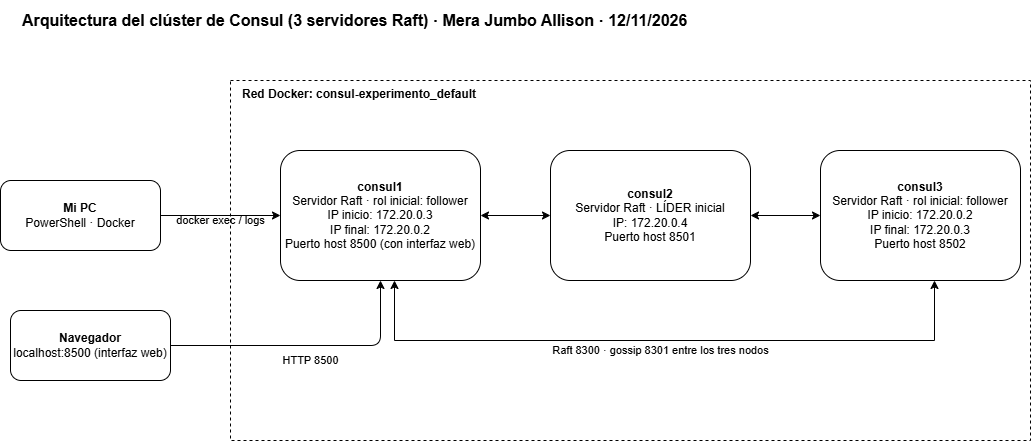
\includegraphics[width=\textwidth]{figuras/arquitectura-consul.png}
  \caption{Arquitectura del clúster de Consul utilizado en el experimento (elaboración propia).}
  \label{fig:arquitectura}
\end{figure}

\subsection{Lectura del diagrama}

La Figura~\ref{fig:arquitectura} muestra tres elementos. El primero es la red Docker, que
contiene los tres servidores con su rol inicial, su dirección IP y el puerto del anfitrión.
consul2 aparece como líder inicial, y consul1 y consul3 como seguidores. El diagrama también
registra que, tras reiniciarse durante el experimento, consul1 y consul3 intercambiaron sus
direcciones IP (de 172.20.0.3 a 172.20.0.2 y de 172.20.0.2 a 172.20.0.3, respectivamente),
mientras que consul2 conservó la suya, 172.20.0.4.

El segundo elemento son los enlaces entre los servidores, representados con flechas dobles y
rotulados con los puertos 8300 y 8301, que son los que aparecen en la configuración de Raft y
en la lista de miembros del clúster en las capturas del experimento. El tercero es lo que queda
fuera de la red Docker: el equipo desde el que se ejecutaron los comandos y se consultaron los
registros de los contenedores, y el navegador, que accede a la interfaz web de consul1.

El boceto del Anexo~A no incluía el cambio de direcciones IP de consul1 y consul3, que se agregó en el diagrama final tras observarlo en el experimento.

\section{Análisis con los conceptos de la Unidad 1}

Los sistemas distribuidos de datos toman decisiones propias en cuanto a consistencia,
tolerancia a fallos y orden de las operaciones \cite{margara2023survey}. Esta sección examina
cuáles tomó Consul, apoyándose en su documentación y en lo observado en el experimento.

\subsection{Transparencias de distribución}


\begingroup
\small
\setlength{\LTpre}{6pt}
\setlength{\LTpost}{6pt}
\setlength{\tabcolsep}{4pt}
\renewcommand{\arraystretch}{1.1}

\begin{longtable}{
    >{\raggedright\arraybackslash}p{2.6cm}
    >{\raggedright\arraybackslash}p{2.4cm}
    >{\raggedright\arraybackslash}p{
        \dimexpr\textwidth-5cm-6\tabcolsep\relax
    }
}

    \caption{Transparencias de distribución en Consul.}
    \label{tab:transparencias}\\

    \toprule
    Transparencia & ¿La ofrece? & Justificación \\
    \midrule
    \endfirsthead

    % Encabezado para las páginas siguientes
    \multicolumn{3}{c}{
        \small Tabla \thetable\ (continuación)
    }\\
    \toprule
    Transparencia & ¿La ofrece? & Justificación \\
    \midrule
    \endhead

    % Pie de tabla para las páginas intermedias
    \midrule
    \multicolumn{3}{r}{
        \footnotesize Continúa en la siguiente página
    }\\
    \endfoot

    % Pie de tabla en la última página
    \bottomrule
    \endlastfoot

    Acceso & Sí &
      Ofrece interfaces uniformes: línea de comandos, API HTTP
      y DNS \cite{etcd_why}. Cualquier servidor atiende una
      petición y, si no es el líder, la reenvía
      \cite{consul_consensus}. En el experimento, los mismos
      comandos se ejecutaron indistintamente contra consul1
      y consul2. \\

    \addlinespace[4pt]

    Ubicación & Sí, para los servicios registrados &
      Un registro de servicios permite descubrir instancias
      de forma dinámica, sin direcciones fijas
      \cite{rodrigues2025stress,etcd_why}. En el experimento,
      los servidores se encontraron entre sí por nombre
      de contenedor (\texttt{-retry-join}) y no por
      dirección. \\

    \addlinespace[4pt]

    Migración & Parcial &
      En el experimento, consul1 y consul3 cambiaron de
      dirección IP al reiniciarse y se reincorporaron con
      su mismo identificador de Raft. No se probó mover
      servicios entre nodos, y la documentación consultada
      no lo garantiza. \\

    \addlinespace[4pt]

    Reubicación & No verificada &
      Consiste en mover un recurso mientras está en uso,
      sin que el usuario lo note. No se probó en el
      experimento ni se halló documentación consultada
      que lo garantice. \\

    \addlinespace[4pt]

    Replicación & Sí, con salvedades &
      El estado se replica con Raft: una entrada se confirma
      cuando está almacenada en un quórum, y el cliente no
      necesita saber qué réplica responde
      \cite{consul_consensus}. La transparencia no es total
      en las lecturas: los modos \textit{default} y
      \textit{stale} pueden devolver valores obsoletos
      \cite{consul_consensus}. \\

    \addlinespace[4pt]

    Concurrencia & Parcial &
      Todas las escrituras pasan por el registro replicado
      del líder, una secuencia ordenada de entradas
      \cite{consul_consensus}. En cuanto a los bloqueos,
      la documentación de etcd, que declara un sesgo a
      favor de etcd, indica que el propio Consul advierte
      que su API de bloqueo no es un método infalible
      \cite{etcd_why}. \\

    \addlinespace[4pt]

    Fallos & Parcial &
      Oculta la caída de una minoría de servidores: tras
      detener o matar al líder, el clúster eligió otro,
      conservó los datos y aceptó escrituras con dos de
      tres nodos. No oculta la pérdida del quórum: sin
      líder, las operaciones fallaron con el error
      \texttt{No cluster leader}
      \cite{consul_consensus}. \\

\end{longtable}
\endgroup


En conjunto, Consul ofrece con claridad las transparencias de acceso y de replicación, y la de
ubicación para los servicios que se registran en él. Las de concurrencia y fallos son
parciales, y las de migración y reubicación no pudieron verificarse con las fuentes y las
pruebas de este trabajo. Esta forma de ocultar la distribución está ligada a la decisión de
priorizar la consistencia, que se analiza en la siguiente subsección.

\subsection{CAP y PACELC}

La documentación de Consul afirma que usa un protocolo de consenso, basado en Raft, para
ofrecer consistencia en el sentido de CAP \cite{consul_consensus}. Cuando no hay quórum
disponible, el clúster deja de estar disponible y no puede confirmar nuevas entradas
\cite{consul_consensus}: ante la pérdida de la mayoría, sacrifica disponibilidad para conservar
la consistencia. La documentación también describe el caso de un líder aislado del resto: puede
elegirse un nuevo líder mientras el anterior conserva su arrendamiento, pero no hay riesgo de
\textit{split-brain}, porque el líder anterior no puede confirmar nuevas entradas; solo sus
lecturas podrían ser obsoletas \cite{consul_consensus}.

En el experimento, con dos de los tres servidores detenidos, el servidor restante no pudo
actuar como líder: la lectura normal, la escritura y la consulta de la configuración de Raft
fallaron con el error \texttt{No cluster leader}, mientras que una lectura en modo
\textit{stale} devolvió el último valor conocido. El resultado es coherente con un
comportamiento orientado a la consistencia, con una vía explícita para conservar la
disponibilidad de lectura a costa de datos posiblemente obsoletos \cite{consul_consensus}. Cabe
aclarar que el experimento provocó caídas de nodos y no una partición de red propiamente dicha,
por lo que no permite afirmar cómo se comporta el clúster ante particiones.


PACELC extiende el análisis de CAP al considerar dos escenarios: ante una partición de red (P), el sistema debe elegir entre disponibilidad (A) y consistencia (C); mientras que, en ausencia de partición (E, \textit{else}), se analiza el compromiso entre latencia (L) y consistencia (C).
Este modelo se utiliza como marco conceptual para interpretar las decisiones de diseño de Consul.


Sin partición, Consul expone esa disyuntiva en sus tres modos de lectura
\cite{consul_consensus}. El modo \textit{default} se apoya en el arrendamiento del líder: las
lecturas son rápidas y normalmente fuertemente consistentes, y solo pueden ser obsoletas en una
situación difícil de provocar. El modo \textit{consistent} exige que el líder verifique con un
quórum que sigue siéndolo, lo que añade un viaje de ida y vuelta y, por tanto, latencia a
cambio de lecturas siempre consistentes. El modo \textit{stale} permite que cualquier servidor
responda, con lecturas rápidas y escalables pero posiblemente obsoletas, generalmente a menos de
50 milisegundos del líder. Las escrituras, por su parte, requieren confirmación por un quórum;
con liderazgo estable, un viaje de ida y vuelta a la mitad del clúster, por lo que su
rendimiento depende del disco y de la latencia de red \cite{consul_consensus}.

A partir de lo anterior, este informe interpreta que Consul prioriza la consistencia ante una
partición y que, sin partición, deja al usuario elegir entre latencia y consistencia en cada
consulta. La documentación consultada no clasifica a Consul con PACELC, por lo que esta
clasificación es una interpretación propia. El experimento tampoco midió la latencia de cada
modo de lectura.

\subsection{Modelos de comunicación}

Consul combina varios modelos de comunicación. Entre clientes y servidores es cliente-servidor:
los nodos cliente reenvían sus peticiones a los servidores, y un servidor que recibe una
petición sin ser el líder la reenvía al líder \cite{consul_consensus}. Entre los servidores, la
replicación sigue un esquema de líder y seguidores: el líder ingiere las entradas nuevas y las
replica en los seguidores \cite{consul_consensus}. Además de la API HTTP, ofrece una interfaz
DNS \cite{etcd_why}.

Desde el punto de vista del cliente, las escrituras son síncronas: bloquean hasta que la
entrada se confirma y se aplica \cite{consul_consensus}. En el experimento, las pruebas se
hicieron con la interfaz de línea de comandos de Consul dentro de los contenedores, y la
interfaz web se consultó por el puerto 8500 del anfitrión.

\subsection{Tolerancia a fallos}

\textbf{Fallos que soporta.} Consul tolera la caída de una minoría de servidores: el consenso
es tolerante a fallos mientras haya quórum, y la tabla de despliegue de la documentación indica
que 3 servidores toleran 1 fallo, 5 toleran 2 y 7 toleran 3, mientras que 1 o 2 servidores no
toleran ninguno \cite{consul_consensus}. No se encontró evidencia de que cubra fallos
bizantinos: trabajos recientes proponen modificar la elección de líder de Raft para resistir
nodos maliciosos \cite{lu2023praft,li2024mec}, lo que sugiere que su diseño original no cubre ese
caso.

\textbf{Detección.} En Raft, si un nodo no recibe entradas del líder durante cierto tiempo, se
promueve a candidato y solicita votos \cite{consul_consensus}. En los registros del
experimento, tras matar a consul1, consul2 registró fallos al enviarle latidos, el módulo de
membresía lo marcó como fallido al agotarse el tiempo de sospecha sin confirmaciones, y
Autopilot, con la limpieza de servidores muertos activada, lo retiró de la configuración de
Raft. En la lista de miembros, consul1 apareció como \texttt{left} y no como \texttt{failed};
este informe no determinó la causa de esa diferencia.

\textbf{Recuperación.} Tras la caída del líder, los servidores restantes eligieron uno nuevo
sin intervención manual, y las escrituras continuaron con dos de tres nodos. Al reiniciar los
contenedores, los nodos se reincorporaron como seguidores y alcanzaron el mismo índice de
confirmación que el líder, sin retraso. Al recuperarse el quórum después de la prueba de
pérdida de mayoría, el clúster recuperó su líder y volvió a aceptar escrituras. El detalle de
estas pruebas se presenta en la sección de Experimentación propia.

\textbf{Incidente documentado.} No se encontró, en las fuentes revisadas, un incidente real de
Consul documentado con una fuente verificable, por lo que esta subsección se apoya en el
experimento propio.

% ==================== 4. EXPERIMENTACIÓN ====================
\section{Experimentación propia}

\subsection{Entorno}

El experimento se realizó el 12 de noviembre de 2026 en un equipo con Windows (PowerShell 5.1),
16~GB de memoria y Docker 29.9.3 con Docker Desktop 4.99.0. Se usó la imagen
\texttt{hashicorp/consul:1.20}, cuyos nodos reportaron la versión 1.20.6. Antes de levantar el
clúster se comprobó el funcionamiento de Docker con la imagen \texttt{hello-world}
(Figura~\ref{fig:captura1}). El clúster se definió con Docker Compose, con tres servidores
(consul1, consul2 y consul3), como se describe en la sección de Arquitectura.

\begin{figure}[H]
  \centering
  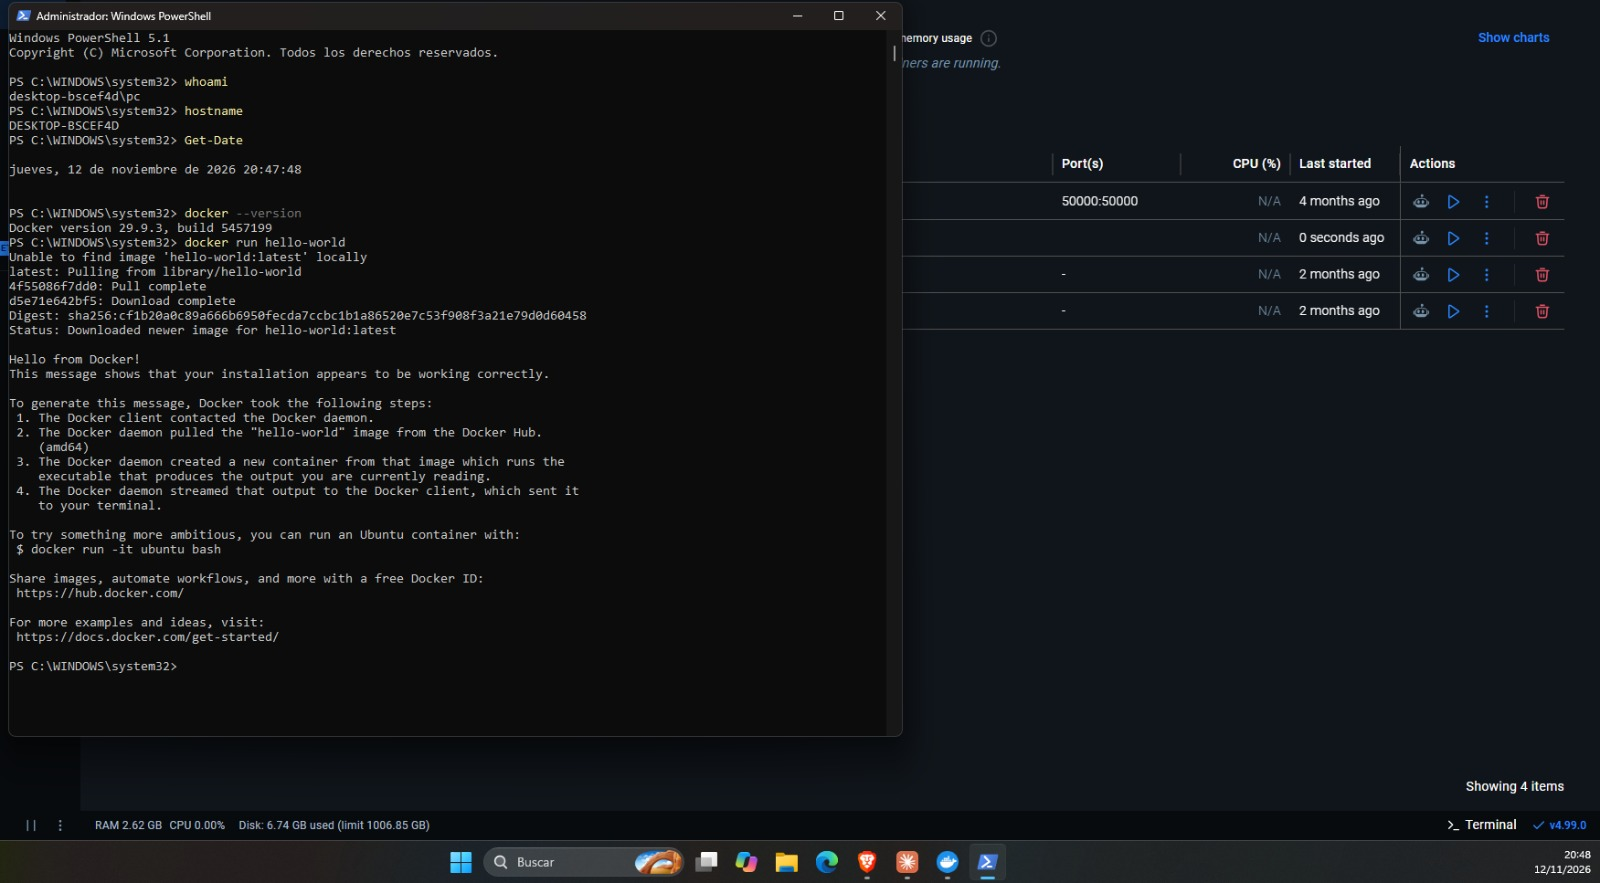
\includegraphics[width=0.95\textwidth]{capturas/01-docker-hello-world.png}
  \caption{Verificación de Docker en el equipo del estudiante. Se observan el usuario, el
  nombre de la máquina, la fecha y hora, la versión de Docker y el mensaje de
  \texttt{hello-world}.}
  \label{fig:captura1}
\end{figure}

\subsection{Procedimiento}

Las pruebas se ejecutaron desde PowerShell con \texttt{docker exec} sobre los contenedores y se
registraron con la transcripción de la consola (\texttt{Start-Transcript}) desde la línea base.
Los comandos y las salidas completos están en el repositorio, en la carpeta
\texttt{experimento} (\url{https://github.com/ameraj2-bit/ta-ind-01-sistemas-distribuidos/tree/main/mera-jumbo-allison/experimento}).
La Tabla~\ref{tab:pruebas} resume las pruebas.

\begin{table}[H]
  \centering
  \small
  \caption{Resumen de las pruebas realizadas.}
  \label{tab:pruebas}
  \begin{tabularx}{\textwidth}{>{\raggedright\arraybackslash}p{0.8cm}>{\raggedright\arraybackslash}p{4.6cm}>{\raggedright\arraybackslash}X}
    \toprule
    Prueba & Acción & Resultado observado \\
    \midrule
    A & Línea base: escritura y lectura de una clave con el clúster sano &
      Líder inicial: consul2. Dato guardado y leído correctamente. \\
    B & \texttt{docker stop} sobre el líder (consul2) &
      Nuevo líder: consul1. El dato se conservó y se aceptó una escritura con 2 de 3 nodos.
      consul2 apareció como \texttt{left}. \\
    C & Reinicio de consul2 &
      Se reincorporó como seguidor, con el mismo índice de confirmación que los demás. \\
    D & \texttt{docker kill} sobre el líder (consul1) &
      Nuevo líder: consul2. consul1 salió de la configuración de Raft por la acción de
      Autopilot y apareció como \texttt{left}. \\
    E & Reinicio de consul1 &
      Se reincorporó solo, como seguidor, con otra dirección IP y el mismo identificador de Raft. \\
    F & \texttt{docker kill} sobre dos de los tres servidores &
      Sin líder: escritura, lectura normal y consulta de Raft fallaron con
      \texttt{No cluster leader}. La lectura \textit{stale} sí respondió. \\
    G & Reinicio de los dos servidores &
      El clúster recuperó su líder y aceptó escrituras de nuevo. \\
    \bottomrule
  \end{tabularx}
\end{table}

La diferencia entre \texttt{docker stop} y \texttt{docker kill} es que el primero solicita al
proceso que termine, mientras que el segundo lo termina de inmediato. Por eso se usaron ambos:
el primero para provocar una salida ordenada del líder y el segundo para una caída abrupta.

\subsection{Resultados}

\textbf{Clúster levantado.} Con los tres contenedores en ejecución, los tres miembros aparecieron
como \texttt{alive} y la configuración de Raft mostró a consul2 como líder y a consul1 y consul3
como seguidores (Figura~\ref{fig:captura2}).

\begin{figure}[H]
  \centering
  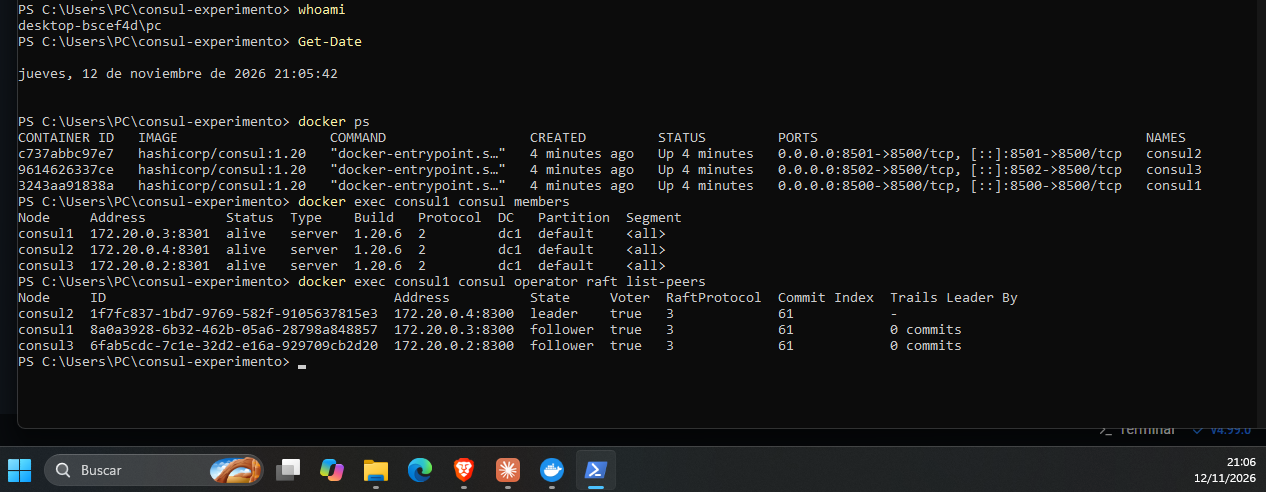
\includegraphics[width=0.95\textwidth]{capturas/02-consul-cluster-levantado.png}
  \caption{Clúster de tres servidores en ejecución: contenedores, miembros y configuración de
  Raft, con consul2 como líder.}
  \label{fig:captura2}
\end{figure}

\textbf{Detención del líder.} Tras detener a consul2, la configuración de Raft mostró solo a
consul1 y consul3, con consul1 como líder. La clave guardada antes de la falla siguió disponible
y se pudo escribir un valor nuevo con dos de tres nodos (Figura~\ref{fig:captura4}).

\begin{figure}[H]
  \centering
  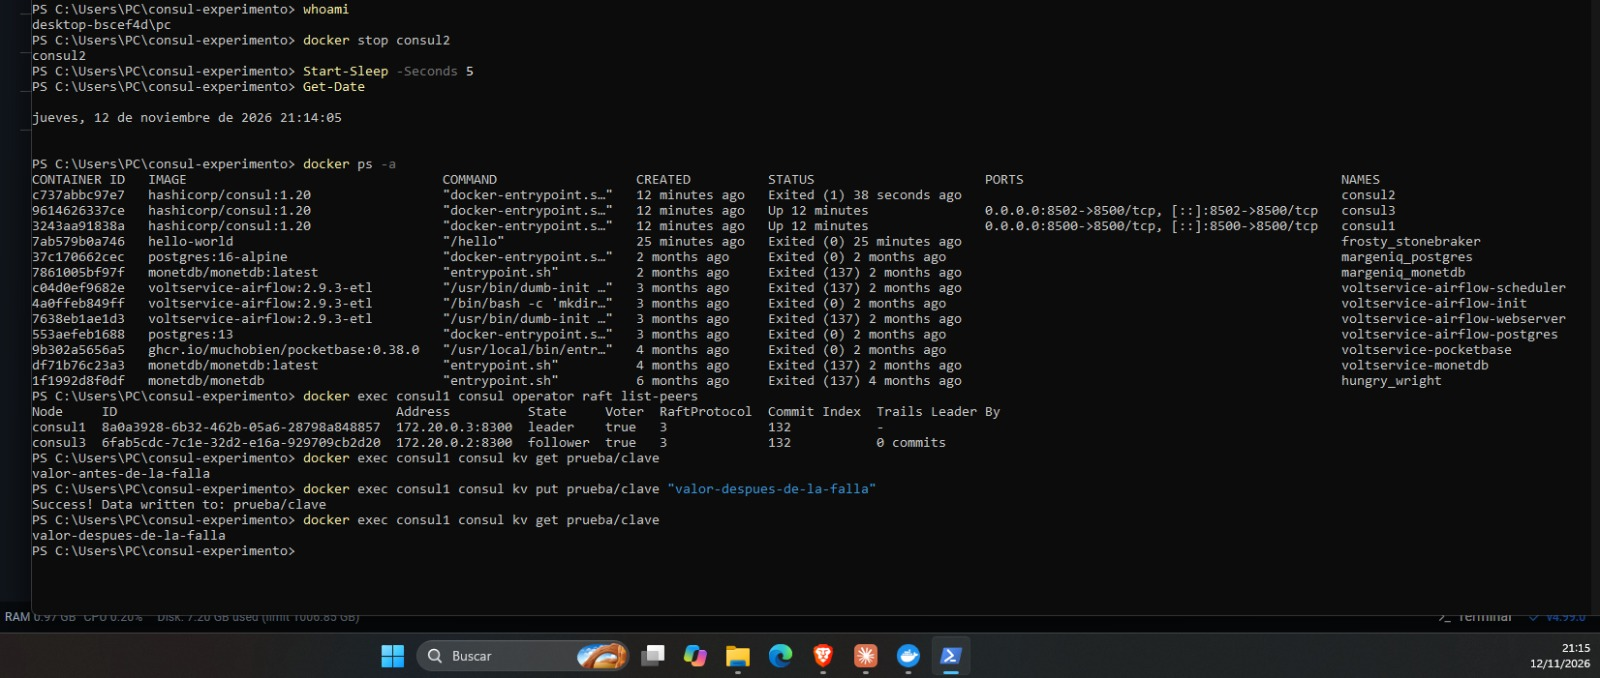
\includegraphics[width=0.95\textwidth]{capturas/04-consul-lider-detenido.png}
  \caption{Estado del clúster después de detener a consul2: nuevo líder, lectura del dato
  previo y escritura con dos de tres nodos.}
  \label{fig:captura4}
\end{figure}

\textbf{Caída abrupta del líder.} Con consul2 reincorporado y consul1 como líder, se mató a
consul1 con \texttt{docker kill}. Cinco segundos después, consul2 era el nuevo líder, y consul1
había salido de la lista de Raft y figuraba como \texttt{left}
(Figura~\ref{fig:captura6}).

\begin{figure}[H]
  \centering
  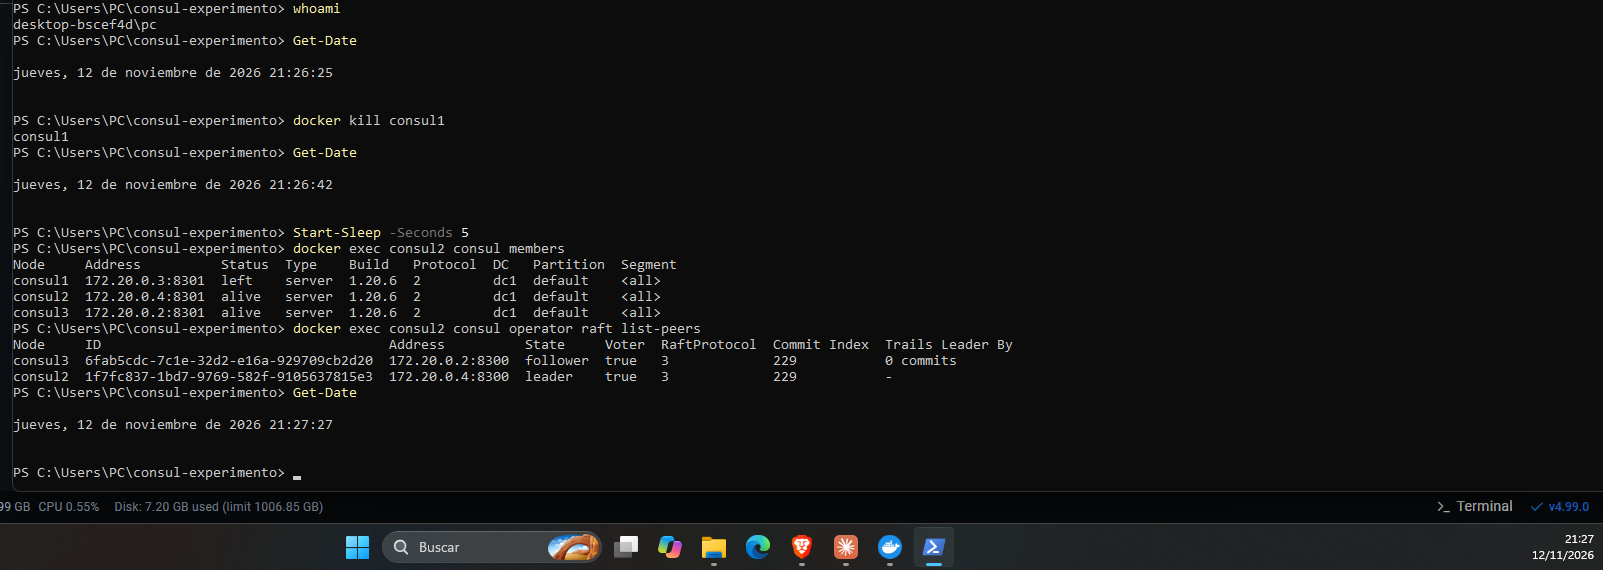
\includegraphics[width=0.95\textwidth]{capturas/06-consul-falla-real.png}
  \caption{Estado del clúster después de matar a consul1: nuevo líder y lista de miembros y de
  Raft con tres horas de referencia.}
  \label{fig:captura6}
\end{figure}

\textbf{Registros de Autopilot.} La configuración de Autopilot tenía activada la limpieza de
servidores muertos (\texttt{CleanupDeadServers = true}). Los registros de consul2 muestran los
fallos al enviar latidos a consul1 y, después, el intento de retirarlo como servidor fallido y
la actualización de la configuración de Raft con el comando \texttt{RemoveServer}
(Figura~\ref{fig:captura7}).

\begin{figure}[H]
  \centering
  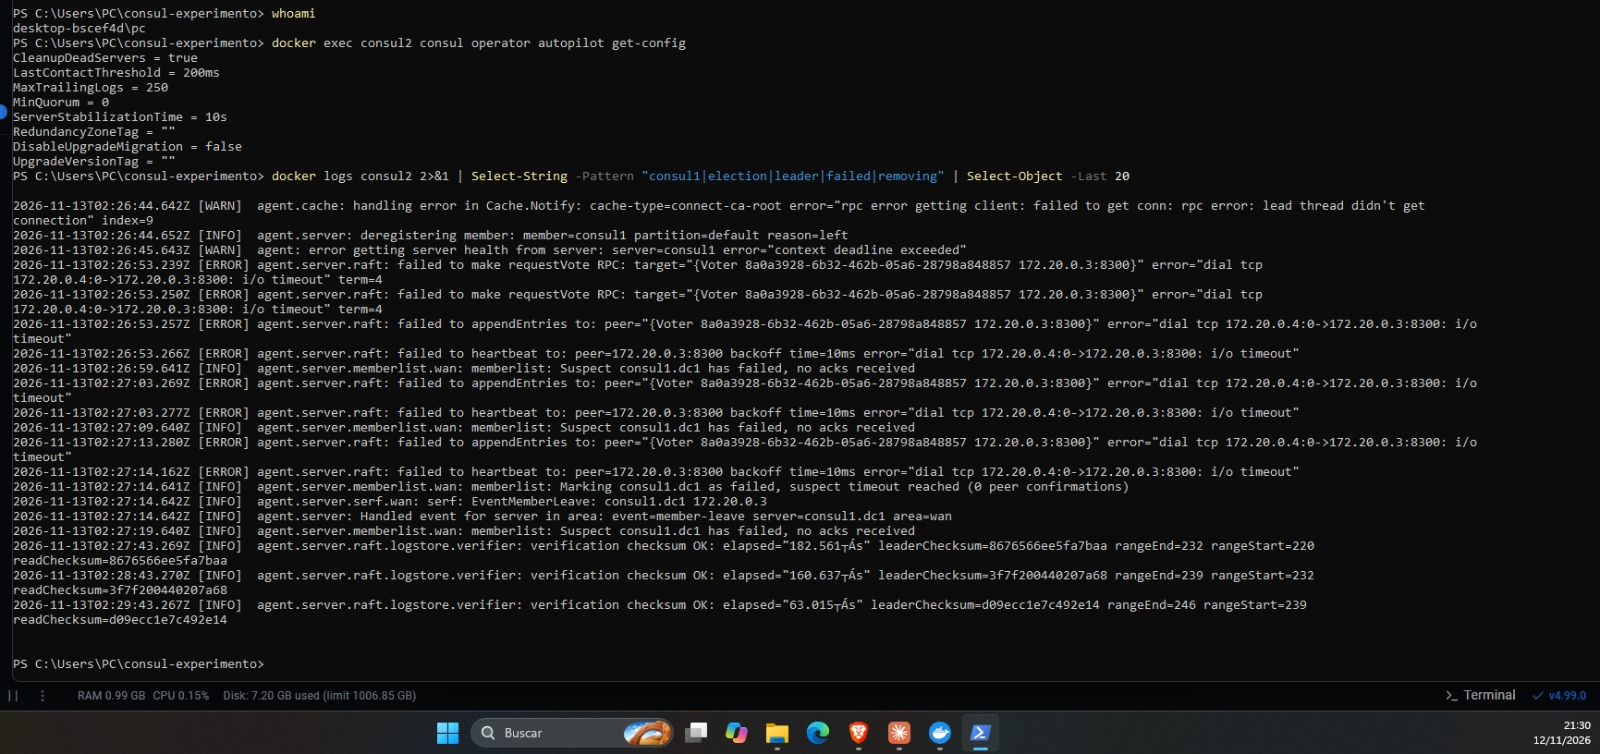
\includegraphics[width=0.95\textwidth]{capturas/07-consul-autopilot-logs.png}
  \caption{Configuración de Autopilot y registros de consul2 sobre la elección y la retirada de
  consul1.}
  \label{fig:captura7}
\end{figure}

\textbf{Tiempo hasta el nuevo líder.} Docker registró que consul1 terminó a las 02:26:34.235
UTC (Figura~\ref{fig:captura9}). El registro de consul2 muestra la activación de la
reconciliación de Autopilot a las 02:26:43.265 UTC y la retirada de consul1 a las 02:26:44.642 UTC.
Si se interpreta la primera como el momento en que consul2 asumió el liderazgo, el tiempo
transcurrido fue de unos 9 segundos. Es una sola medición, con una interpretación propia que no
se verificó en la documentación.

\begin{figure}[H]
  \centering
  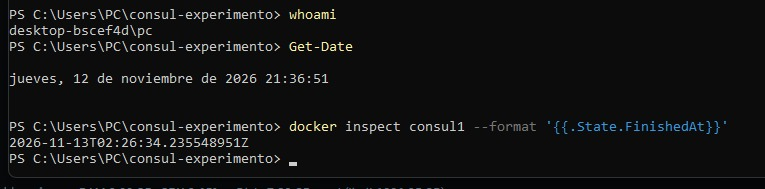
\includegraphics[width=0.95\textwidth]{capturas/09-consul-finishedat.png}
  \caption{Hora de término de consul1 según Docker (UTC).}
  \label{fig:captura9}
\end{figure}

\textbf{Pérdida del quórum.} Al matar a consul1 y consul3 a la vez, el servidor restante
(consul2) no pudo actuar como líder. La consulta de la configuración de Raft, la escritura y la
lectura normal fallaron con el error 500 \texttt{No cluster leader}, mientras que la lectura en
modo \textit{stale} devolvió el último valor guardado (Figura~\ref{fig:captura11}).

\begin{figure}[H]
  \centering
  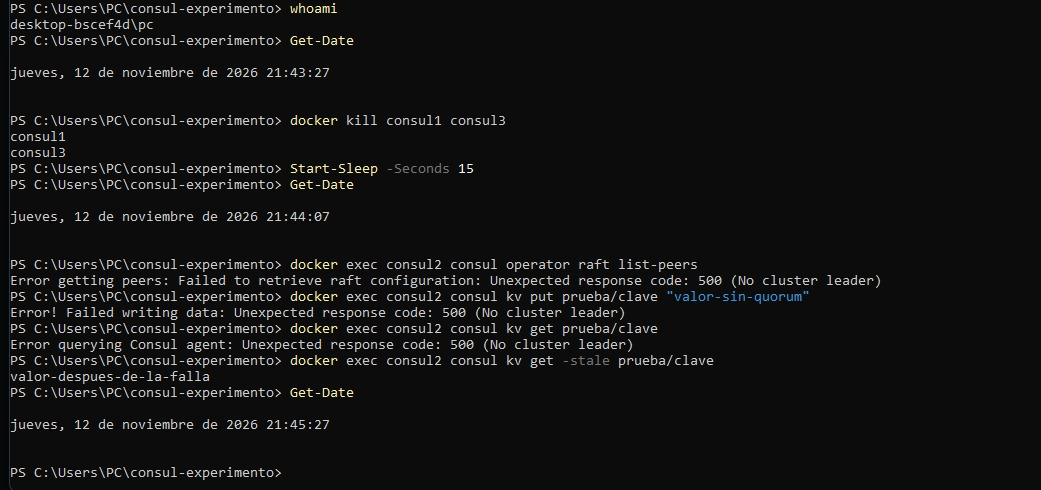
\includegraphics[width=0.95\textwidth]{capturas/11-consul-sin-quorum.png}
  \caption{Clúster con dos de tres servidores caídos: fallos de escritura y lectura normal, y
  lectura \textit{stale} exitosa.}
  \label{fig:captura11}
\end{figure}

\textbf{Recuperación.} Al reiniciar consul1 y consul3, los tres miembros volvieron a estar
\texttt{alive}, hubo líder de nuevo (consul2), los tres nodos mostraron el mismo índice de
confirmación y se aceptó una escritura (Figura~\ref{fig:captura12}). Las capturas restantes
del experimento están en el repositorio.

\begin{figure}[H]
  \centering
  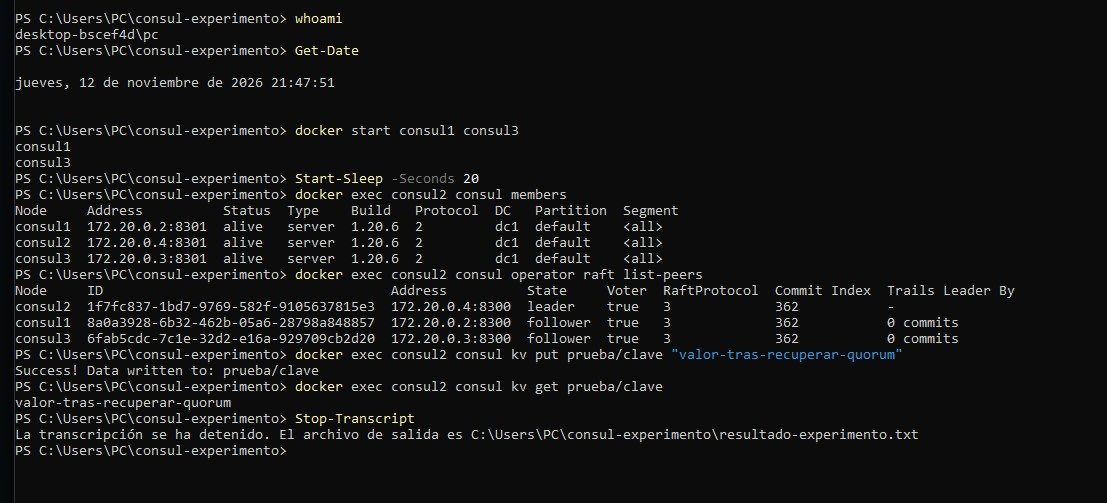
\includegraphics[width=0.95\textwidth]{capturas/12-consul-quorum-recuperado.png}
  \caption{Clúster recuperado tras reiniciar los dos servidores: miembros, líder y nueva
  escritura.}
  \label{fig:captura12}
\end{figure}

\subsection{Interpretación}

\textbf{Pérdida de un servidor.} En las pruebas B y D, el clúster siguió funcionando tras perder
a su líder, ya fuera detenido o muerto: los dos servidores restantes eligieron uno nuevo, el
dato se conservó y se pudo escribir. Es lo esperable de Raft, cuyo consenso tolera fallos
mientras haya quórum, y con tres servidores el quórum es de dos \cite{consul_consensus}. Con
una sola medición en un único equipo, el tiempo hasta el nuevo líder (unos 9 segundos en la
prueba D) no permite generalizar.

\textbf{Detención frente a caída.} Ambas pruebas terminaron con el servidor caído fuera de la
configuración de Raft y marcado como \texttt{left}. En la prueba D, los registros indican que
fue Autopilot, con la limpieza de servidores muertos activada, quien lo retiró. Este informe no
determinó por qué la lista de miembros mostró \texttt{left} en lugar de \texttt{failed}.

\textbf{Reincorporación.} En las pruebas C y E, los servidores se reincorporaron solos como
seguidores y alcanzaron el mismo índice de confirmación que el líder, sin retraso. En la
prueba E, consul1 regresó con otra dirección IP y el mismo identificador de Raft, lo que
sugiere que el clúster lo reconoce por su identificador y no por su dirección. Es una lectura
propia de lo observado.

\textbf{Pérdida del quórum.} En la prueba F, con dos de tres servidores caídos, el clúster
dejó de aceptar escrituras y lecturas normales. La documentación indica que, si no hay quórum,
el clúster deja de estar disponible y no puede confirmar nuevas entradas, y que el modo
\textit{stale} permite que un servidor responda aun sin líder \cite{consul_consensus}. Ambos
comportamientos coinciden con lo observado. El valor devuelto por la lectura \textit{stale} no
estaba desactualizado, porque no se había confirmado ninguna escritura posterior, así que la
prueba no muestra lectura de datos obsoletos.

En términos de CAP, estas observaciones son coherentes con un sistema que, ante la pérdida de
la mayoría, sacrifica la disponibilidad de escritura para conservar la consistencia, con la
lectura \textit{stale} como vía explícita para conservar la disponibilidad de lectura a costa
de consistencia. Sin embargo, el experimento provocó caídas de nodos y no una partición de red,
y no midió la latencia de cada modo de lectura, por lo que no ilustra la disyuntiva de PACELC
cuando no hay partición.

\textbf{Limitaciones.} Cada prueba se ejecutó una sola vez, en un único equipo y con
contenedores de Docker, por lo que los resultados no representan un despliegue en producción.
Las pruebas B y D se hicieron comando por comando, así que los intervalos entre
\texttt{Get-Date} incluyen el tiempo de escritura del propio estudiante y solo permiten
acotar los tiempos.


% ==================== 5. EJEMPLOS DEL ENTORNO ====================
\section{Ejemplos del entorno del estudiante}

Esta sección relaciona dos sistemas que el estudiante ha usado de primera mano con conceptos de
la Unidad~1. En ambos casos lo observado proviene de la experiencia como usuario, y no se
conoce la arquitectura interna de estos sistemas, por lo que las explicaciones son
interpretaciones y no afirmaciones sobre cómo están construidos.

\subsection{Sistema de Gestión Académica (SGA) en la semana de matrículas}

\textbf{Observación.} Durante la semana de matrículas, la
sección de matrícula del SGA se caía y se demoraba mucho cada vez que se intentaba agregar una
asignatura. La información tardaba en reflejarse y, en la práctica, dejaba de estar disponible.

\textbf{Concepto relacionado.} Lo observado se relaciona con la disponibilidad: durante un
periodo de alta demanda, el sistema dejó de responder o respondió con mucha demora. También se
relaciona con la transparencia de fallos, que busca que el usuario no perciba los problemas
internos del sistema; aquí el fallo fue visible. Una posible explicación es la sobrecarga por
muchas solicitudes simultáneas, pero sin conocer la arquitectura del SGA no puede afirmarse
cuál fue la causa.

\textbf{Relación con el experimento.} En el experimento con Consul, al perderse el quórum, las
operaciones fallaron de inmediato con un mensaje de error explícito (\texttt{No cluster
leader}) y se conocía la causa, porque la provocó el propio estudiante. En el SGA, en cambio,
la operación se demoraba sin que se supiera el motivo. En ambos casos el usuario perdió el
acceso a una función, aunque con diferente información sobre el fallo.

\subsection{WhatsApp y los servicios de Meta}

\textbf{Observación.} El servicio de WhatsApp dejó de funcionar:
los mensajes no se enviaban ni se recibían. Al principio no se  podía saber si el
problema era la conexión Wi-Fi o el servicio. Al mismo tiempo ocurría lo mismo con Facebook, y
se supo después que habían caído varios servicios de Meta a la vez.

\textbf{Concepto relacionado.} Es un caso de pérdida de disponibilidad. Muestra además la
dificultad de distinguir, desde el lado del cliente, un fallo de la propia red de un fallo del
servicio, porque ambos se manifiestan igual: los mensajes no salen. Que varios servicios
cayeran simultáneamente sugiere que compartían alguna parte de su infraestructura, pero esto es
una inferencia y no un dato confirmado. 

\textbf{Relación con el experimento.} En el experimento, la pérdida de un servidor fue
absorbida por el clúster: la falla de una minoría no impidió seguir escribiendo. La pérdida de
la mayoría, en cambio, sí interrumpió el servicio, de modo parecido a lo vivido con WhatsApp,
donde la interrupción fue total. La diferencia es que en el clúster de Consul el error
indicaba la causa, mientras que el usuario de WhatsApp no tenía forma de saberla.
% ==================== 6. ANÁLISIS COMPARATIVO ====================

\section{Análisis comparativo}

Esta sección compara Consul con etcd, un almacén clave-valor
distribuido que también usa Raft.
Hay una diferencia de método: Consul se analizó con un
experimento propio, mientras que etcd se estudió solo con
su documentación y con trabajos publicados, sin ejecutarlo.

\begingroup
\small
\setlength{\LTpre}{6pt}
\setlength{\LTpost}{6pt}
\setlength{\tabcolsep}{4pt}
\renewcommand{\arraystretch}{1.1}

\begin{longtable}{
    >{\raggedright\arraybackslash}p{2.4cm}
    >{\raggedright\arraybackslash}p{
        \dimexpr(\textwidth-2.4cm-6\tabcolsep)/2\relax
    }
    >{\raggedright\arraybackslash}p{
        \dimexpr(\textwidth-2.4cm-6\tabcolsep)/2\relax
    }
}

    \caption{Comparación entre Consul y etcd.}
    \label{tab:comparacion}\\

    \toprule
    Criterio & Consul & etcd \\
    \midrule
    \endfirsthead

    % Encabezado para las páginas siguientes
    \multicolumn{3}{c}{
        \small Tabla \thetable\ (continuación)
    }\\
    \toprule
    Criterio & Consul & etcd \\
    \midrule
    \endhead

    % Pie de tabla para las páginas intermedias
    \midrule
    \multicolumn{3}{r}{
        \footnotesize Continúa en la siguiente página
    }\\
    \endfoot

    % Pie de tabla en la última página
    \bottomrule
    \endlastfoot

    Prioridad en CAP &
      Usa consenso (Raft) para ofrecer consistencia en el
      sentido de CAP; sin quórum, el clúster no está
      disponible \cite{consul_consensus}. En el experimento,
      sin quórum fallaron las escrituras. &
      Se describe como una base para sistemas que no
      toleran el \textit{split-brain} y están dispuestos
      a sacrificar disponibilidad \cite{etcd_why}.
      Misma orientación a la consistencia. \\

    \addlinespace[4pt]

    Prioridad en PACELC &
      Tres modos de lectura: \textit{default} (rápido,
      casi siempre consistente), \textit{consistent}
      (consistente, con un viaje extra) y \textit{stale}
      (rápido, posiblemente obsoleto)
      \cite{consul_consensus}. No se midió la latencia
      de cada modo. &
      Ofrece lecturas linearizables, con una latencia
      mínima de un viaje de red de ida y vuelta;
      para Consul, su documentación indica ese viaje
      más \textit{fsync} \cite{etcd_why}. No se verificó
      si ofrece un modo equivalente a \textit{stale}. \\

    \addlinespace[4pt]

    Modelo de comunicación &
      Cliente-servidor: un servidor que no es el líder
      reenvía la petición al líder; el líder replica
      en los seguidores \cite{consul_consensus}.
      Ofrece API HTTP y DNS \cite{etcd_why}. &
      Protocolo de cliente basado en gRPC, que puede
      expresarse en JSON sobre HTTP; la replicación
      pasa por Raft en un solo grupo
      \cite{etcd_why}. \\

    \addlinespace[4pt]

    Tolerancia a fallos y consenso &
      Raft con quórum de mayoría: 3 servidores toleran
      1 fallo y 5 toleran 2 \cite{consul_consensus}.
      En el experimento, el clúster eligió nuevo líder
      tras perder al líder y no aceptó escrituras al
      perder la mayoría. &
      Raft en un solo grupo de replicación, con
      reconfiguración dinámica de miembros
      \cite{etcd_why}. Su base combina una biblioteca
      de Raft, un registro de escritura anticipada
      y BoltDB \cite{lebow2025smr}. Al usar Raft,
      cabe esperar el mismo principio de mayoría;
      no se probó. \\

    \addlinespace[4pt]

    Transparencias que ofrece &
      Acceso, ubicación y replicación; concurrencia
      y fallos de forma parcial
      (Tabla~\ref{tab:transparencias}). &
      Acceso uniforme por gRPC o HTTP y replicación
      en un solo grupo \cite{etcd_why}. Las demás
      no se verificaron. \\

    \addlinespace[4pt]

    Escala de datos &
      Según la documentación de etcd, una base
      confiable de cientos de MB \cite{etcd_why};
      la de Consul indica del orden de cientos
      a miles de transacciones por segundo
      \cite{consul_consensus}. &
      Varios gigabytes, y su replicación no escala
      horizontalmente porque no particiona los
      datos \cite{etcd_why}. \\

\end{longtable}
\endgroup


Ambos sistemas comparten el mismo fundamento, Raft, y una orientación similar a la consistencia
frente a la disponibilidad. Las diferencias están en el propósito y en las prestaciones. La
documentación de etcd afirma que ambos resuelven problemas distintos: etcd sería mejor como
almacén clave-valor consistente, mientras que Consul es un marco de descubrimiento de servicios
de extremo a extremo, con comprobaciones de salud, detección de fallos y DNS \cite{etcd_why}.
Esa fuente es del equipo de etcd y declara un sesgo a favor de etcd, por lo que sus
valoraciones sobre Consul deben leerse con cautela.

En la práctica, Consul parece más adecuado cuando una aplicación de microservicios necesita
localizar servicios y verificar su salud, como en el caso de uso revisado
\cite{rodrigues2025stress}, y expone de forma explícita la disyuntiva entre latencia y
consistencia en cada lectura \cite{consul_consensus}. etcd parece más adecuado para almacenar
metadatos o coordinar procesos con un orden estricto, y según su documentación, es el almacén
de configuración de Kubernetes \cite{etcd_why}. Esta valoración es una interpretación propia.

Hay tres límites en la comparación. Primero, solo Consul se ejecutó; lo dicho de etcd proviene
de documentación y no se contrastó con un experimento. Segundo, el trabajo de Lebow y
colaboradores describe un sistema inspirado en etcd, no etcd mismo, por lo que se usó solo para
sus componentes y no para sus cifras de rendimiento \cite{lebow2025smr}. Tercero, las
comparaciones de escala provienen de una fuente con sesgo declarado.

% ==================== 7. POSTURA CRÍTICA ====================
\section{Postura crítica}

\subsection{Fortalezas}

\textbf{Consistencia fuerte en las escrituras.} Todas las escrituras de Consul pasan por Raft y
se confirman cuando están almacenadas en un quórum de servidores \cite{consul_consensus}. En el
experimento, el clúster nunca aceptó una escritura sin mayoría: al perder dos de tres
servidores, la escritura falló en lugar de confirmarse sin consenso. Esto evita estados
divergentes, que es la razón de ser del consenso.

\textbf{Tolerancia a la caída de una minoría, sin intervención manual.} Con tres servidores, el
quórum es de dos y se tolera un fallo \cite{consul_consensus}. En el experimento, tanto al
detener como al matar al líder, los servidores restantes eligieron otro, el dato se conservó y
se pudo seguir escribiendo; al reiniciar los contenedores, los nodos se reincorporaron solos.

\textbf{Control sobre la latencia de lectura.} Sus tres modos de lectura permiten elegir, por
consulta, entre rapidez y consistencia \cite{consul_consensus}. Esto evita imponer una única
política a todas las aplicaciones. En el experimento, la lectura \textit{stale} fue la única
que respondió sin líder.

\textbf{Funciones integradas.} Además del almacenamiento, ofrece descubrimiento de servicios,
comprobaciones de salud y DNS \cite{etcd_why}, y se ha usado como registro de servicios en una
arquitectura de microservicios \cite{rodrigues2025stress}. La fuente de las funciones es del
equipo de etcd, con el sesgo ya mencionado.

\subsection{Limitaciones y compromisos}

\textbf{Se sacrifica la disponibilidad de escritura sin quórum.} Si no hay mayoría, el clúster no
puede confirmar nuevas entradas \cite{consul_consensus}, y en el experimento las escrituras y las
lecturas normales fallaron con \texttt{No cluster leader}. Es el precio de la consistencia, y
para una aplicación que deba aceptar escrituras aun sin mayoría, es una limitación seria.

\textbf{Las lecturas por defecto pueden ser obsoletas.} El modo \textit{default} se apoya en el
arrendamiento del líder, y la propia documentación admite que, si el líder queda aislado, sus
lecturas podrían ser obsoletas, aunque lo describe como una situación difícil de provocar
\cite{consul_consensus}. Es un compromiso a favor de la velocidad.

\textbf{El rendimiento de escritura está acotado.} Con liderazgo estable, confirmar una entrada
requiere un viaje de ida y vuelta a la mitad del clúster, por lo que el rendimiento depende del
disco y de la latencia de red, y la documentación advierte que Consul no está diseñado como
sistema de escritura de alto rendimiento \cite{consul_consensus}. Además, solo los servidores
participan en Raft porque, al crecer el conjunto de pares, también crece el quórum y con él los
problemas de rendimiento \cite{consul_consensus}; añadir servidores no aumenta la capacidad de
escritura.

\textbf{La retirada automática reduce el margen de tolerancia.} En el experimento, tras matar a
consul1, Autopilot lo retiró de la configuración de Raft y quedaron dos votantes. Con dos pares,
el quórum es de dos y la caída de cualquiera de ellos impide alcanzarlo
\cite{consul_consensus}. Por tanto, mientras el nodo retirado no regresara, el clúster no habría
tolerado otro fallo. Esta es una interpretación propia, no probada en el experimento.

\textbf{Raft no cubre fallos bizantinos.}
El algoritmo Raft convencional está orientado a tolerar fallos de nodos mediante consenso por mayoría, pero no proporciona garantías frente a comportamientos bizantinos. En este sentido, Li et al. proponen modificar la fase de elección del líder mediante un mecanismo de compartición de secretos y votación, con el propósito de mejorar la resistencia frente a nodos maliciosos \cite{li2024mec}. Esta limitación debe considerarse en entornos donde no se puede confiar plenamente en todos los participantes.


\textbf{Limitaciones del propio análisis.} El experimento se ejecutó una vez, en un equipo, con
Docker, y provocó caídas de nodos pero no particiones de red ni midió la latencia de cada modo
de lectura. Además, no se encontraron cifras públicas de adopción, lo que limita la valoración
de su uso a gran escala.

\subsection{Contextos en los que no sería la mejor opción}

\begin{itemize}
  \item \textbf{Cargas de escritura intensas.} Su documentación lo descarta como sistema de
  escritura de alto rendimiento \cite{consul_consensus}, y la de etcd afirma que su
  almacén es más adecuado que el de Consul para grandes volúmenes de claves
  \cite{etcd_why}, con el sesgo señalado.
  \item \textbf{Aplicaciones que deban aceptar escrituras sin mayoría.} Al priorizar la
  consistencia, se pierde esa disponibilidad.
  \item \textbf{Entornos con nodos no confiables.} Por la ausencia de tolerancia a fallos
  bizantinos, según lo discutido arriba.
  \item \textbf{Despliegues de uno o dos servidores.} La documentación indica que con uno o dos
  servidores no se tolera ningún fallo, y que un solo servidor es muy desaconsejable porque la
  pérdida de datos es inevitable ante una falla \cite{consul_consensus}.
  \item \textbf{Cuando solo se necesita un almacén clave-valor consistente.} La documentación
  de etcd recomienda etcd para ese caso y Consul para el descubrimiento de servicios
  \cite{etcd_why}, otra vez con sesgo a favor de etcd.
\end{itemize}



% ==================== 8. CONCLUSIONES ====================
\section{Conclusiones}

\begin{enumerate}
  \item \textbf{El clúster de tres servidores siguió operando tras perder a su líder, tanto en una detención ordenada como en una caída abrupta.} En ambas pruebas se eligió un nuevo líder entre los dos servidores restantes, el dato guardado antes de la falla se conservó y se aceptó una escritura con dos de tres nodos. En la caída abrupta, el nuevo líder apareció unos 9 segundos después de que Docker registrara el fin del contenedor. Es una sola medición, en un equipo y con contenedores, por lo que no permite generalizar el tiempo.

  \item \textbf{Sin mayoría de servidores, Consul rechazó las escrituras y las lecturas
  normales, y solo respondió una lectura \textit{stale}.} Con dos de tres servidores caídos, la escritura, la lectura normal y la consulta de la configuración de Raft fallaron con el error \texttt{No cluster leader}, mientras que la lectura en modo \textit{stale} devolvió el último valor guardado. Esto es coherente con una prioridad de la consistencia sobre la disponibilidad de escritura. El experimento provocó caídas de nodos y no particiones de red, así que no muestra cómo se comporta ante una partición.

  \item \textbf{La retirada automática de un servidor caído cambió la composición del clúster sin
  intervención manual.} Tras matar a consul1, Autopilot lo retiró de la configuración de Raft y la lista de miembros lo mostró como \texttt{left}. Al reiniciarlo, consul1 volvió solo como seguidor, con una dirección IP distinta y el mismo identificador de Raft. Este informe no determinó por qué apareció como \texttt{left} y no como \texttt{failed}, y no probó qué habría ocurrido ante un segundo fallo mientras el clúster quedaba con dos votantes.

  \item \textbf{Frente a etcd, Consul comparte la base de consenso, pero cambia el propósito.}
  La documentación revisada presenta a etcd como almacén clave-valor consistente y a Consul como marco de descubrimiento de servicios. Lo dicho de etcd proviene de
  documentación con sesgo declarado y no se contrastó con un experimento, por lo que la
  comparación es una valoración preliminar. Una prueba equivalente sobre etcd permitiría
  contrastarla.
\end{enumerate}

% ==================== 9. DECLARACIÓN DE USO DE IA ====================
\section{Declaración de uso de inteligencia artificial}

\textbf{Herramientas.} Se utilizaron dos asistentes de inteligencia artificial generativa:
Claude, de Anthropic (Claude Sonnet 5.5), y ChatGPT, de OpenAI
(GPT-6).

\textbf{Para qué se usaron.} Claude se usó para guiar la creación del repositorio y su
estructura en GitHub; para proponer el esqueleto del documento LaTeX; para entregar los comandos y el archivo \texttt{docker-compose.yml} del clúster de Consul, que el estudiante ejecutó; para revisar los campos del archivo BibTeX. ChatGPT se usó para la correción ortográfica y gramática.


\textbf{Responsabilidad.} El estudiante asume la responsabilidad del contenido del informe, incluidos los posibles errores de los textos generados en la correciones gramáticales.
\newpage

% ==================== REFERENCIAS ====================
\printbibliography[title={Referencias}]

% ==================== ANEXOS ====================
\clearpage
\section*{Anexo A: esquema inicial a mano}
\addcontentsline{toc}{section}{Anexo A: esquema inicial a mano}
\begin{figure}[H]
  \centering
  \includegraphics[width=0.9\textwidth]{figuras/anexo-a-esquema-mano.png}
  \caption{Primer bosquejo de la arquitectura de Consul, dibujado a mano por el estudiante.}
\end{figure}

\clearpage


\section*{Anexo B: capturas de lectura de las fuentes}
\addcontentsline{toc}{section}{Anexo B: capturas de lectura de las fuentes}

% ==================== CAPTURA 1 ====================

\begin{figure}[H]
    \centering
    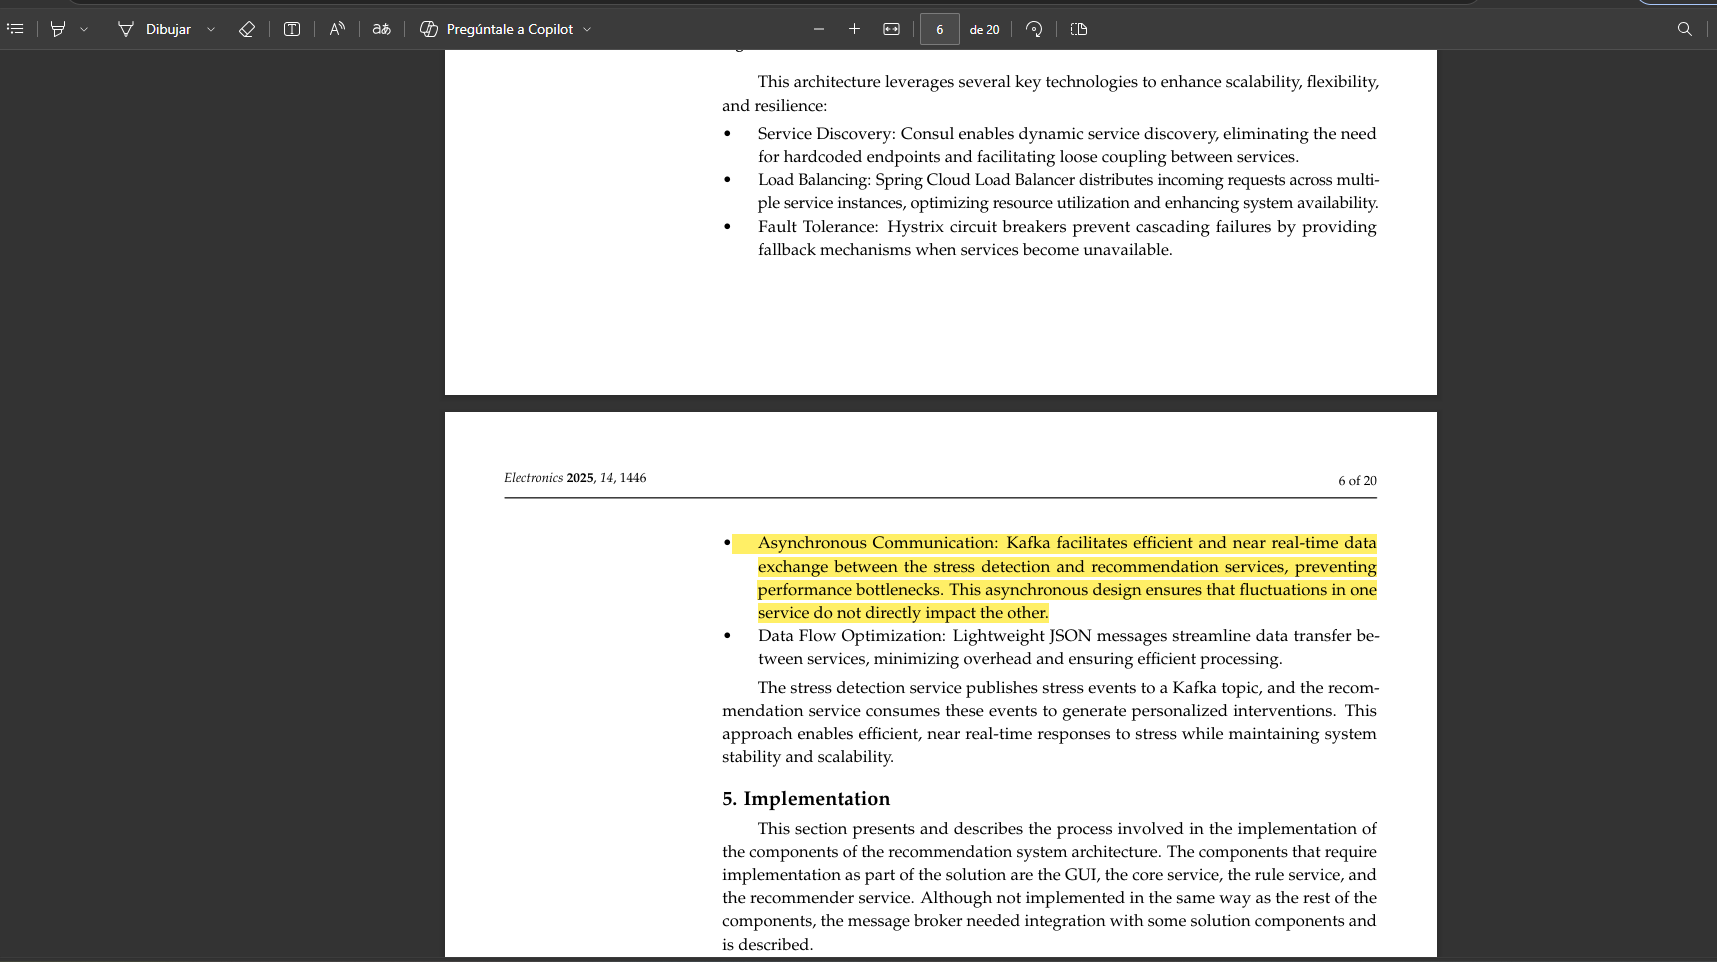
\includegraphics[width=0.9\textwidth]{capturas/lectura-1.png}
    \caption{Comunicación asíncrona mediante Kafka.
    Rodrigues et al. (2025), página 6, sección 4,
    apartado Asynchronous Communication.
    El fragmento subrayado describe el intercambio
    asíncrono de información entre los servicios
    de detección de estrés y recomendación.
    Esta información se cita en la sección
    Introducción del presente informe, en el
    segundo párrafo: ``un sistema de recomendación
    lo usa para evitar direcciones fijas entre
    servicios, junto con Kafka para la comunicación
    asíncrona'' \cite{rodrigues2025stress}.}
    \label{fig:lectura-kafka}
\end{figure}


% ==================== CAPTURA 2 ====================

\begin{figure}[H]
    \centering
    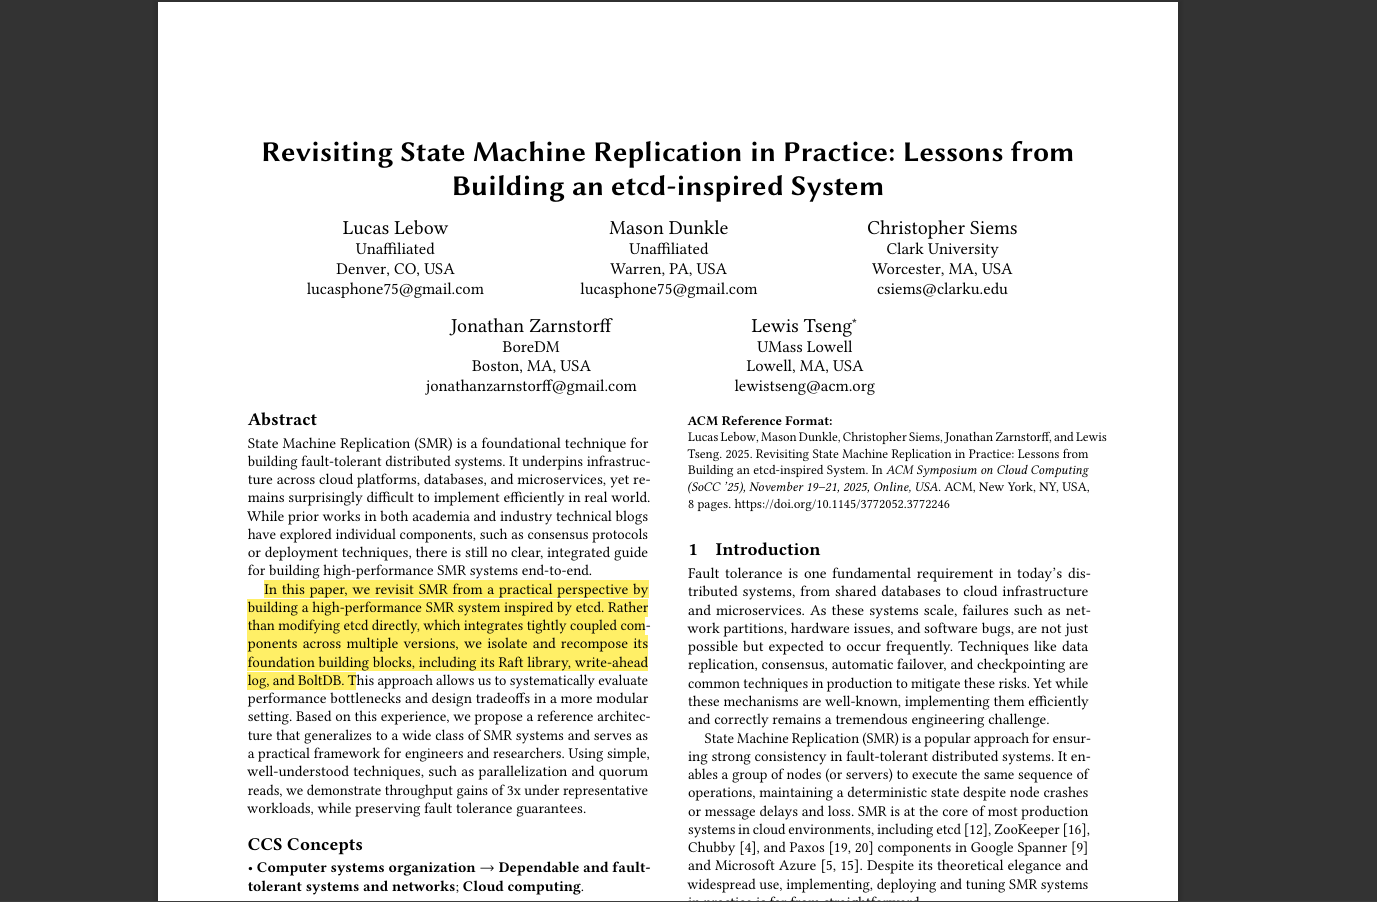
\includegraphics[width=0.9\textwidth]{capturas/lectura-2.png}
    \caption{Componentes de un sistema inspirado en etcd.
    Lebow et al. (2025), página 456, sección Abstract,
    segundo párrafo. El fragmento subrayado identifica
    la biblioteca Raft, el registro de escritura
    anticipada (WAL) y BoltDB, y aclara que no se
    modificó directamente etcd.
    Esta información se cita en la sección
    Análisis comparativo, en la tabla
    Comparación entre Consul y etcd, criterio
    Tolerancia a fallos y consenso, columna etcd:
    ``Su base combina una biblioteca de Raft,
    un registro de escritura anticipada y BoltDB''.
    También se cita en el último párrafo de la
    sección: ``el trabajo de Lebow y colaboradores
    describe un sistema inspirado en etcd, no etcd
    mismo'' \cite{lebow2025smr}.}
    \label{fig:lectura-lebow}
\end{figure}


% ==================== CAPTURA 3 ====================

\begin{figure}[H]
    \centering
    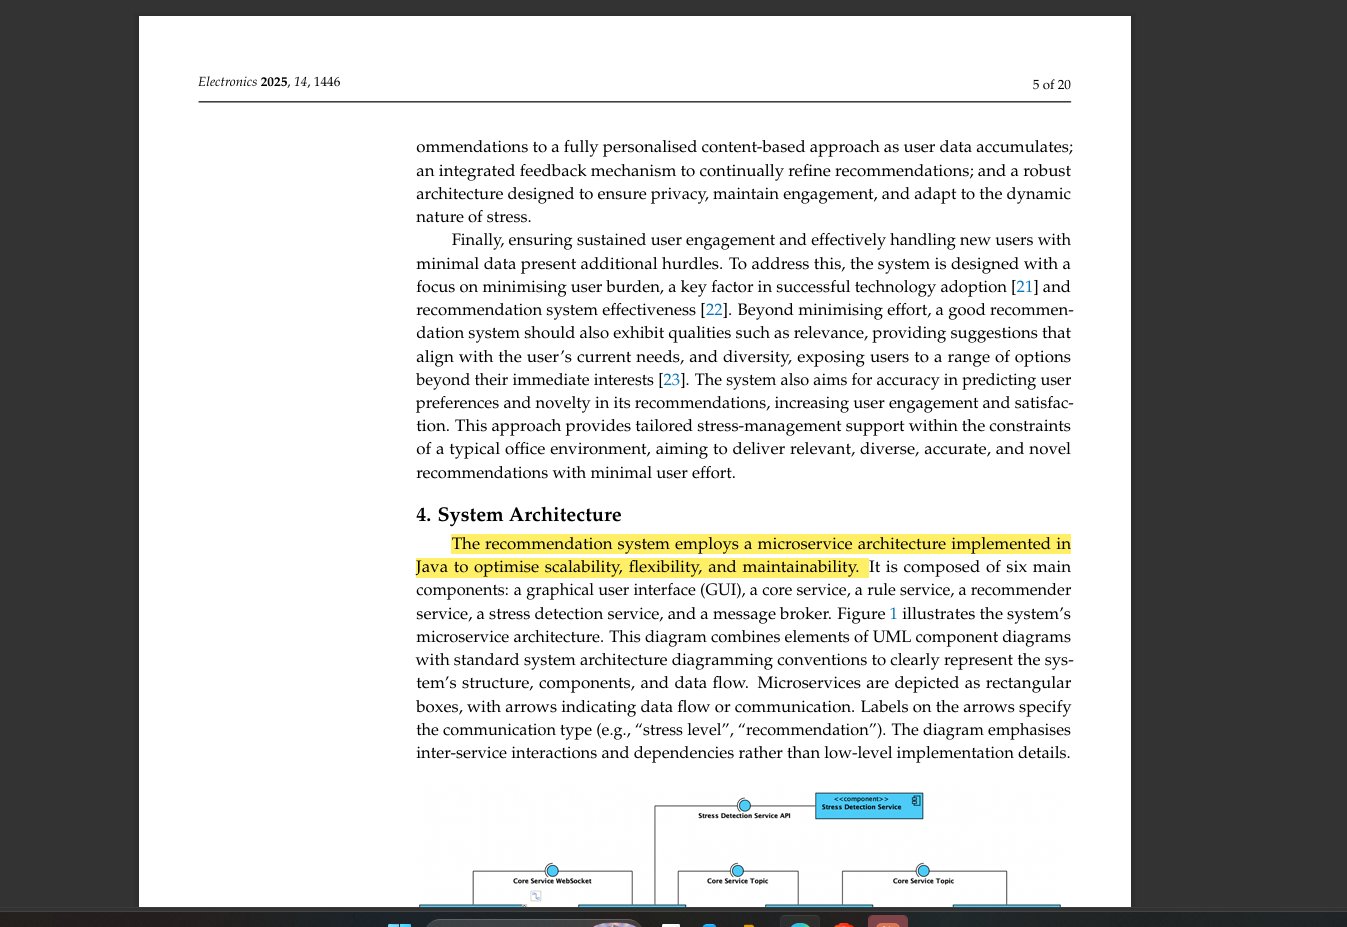
\includegraphics[width=0.9\textwidth]{capturas/lectura-3.png}
    \caption{Arquitectura de microservicios implementada
    en Java. Rodrigues et al. (2025), página 5,
    sección 4, System Architecture, primer párrafo.
    El fragmento subrayado describe una arquitectura
    orientada a mejorar la escalabilidad, flexibilidad
    y mantenibilidad.
    Esta información se relaciona con la sección
    Análisis comparativo, en el párrafo posterior
    a la tabla Comparación entre Consul y etcd:
    ``En la práctica, Consul parece más adecuado
    cuando una aplicación de microservicios necesita
    localizar servicios y verificar su salud,
    como en el caso de uso revisado''.
    El uso específico de Consul se explica en el
    apartado Service Discovery, página 5,
    del mismo artículo \cite{rodrigues2025stress}.}
    \label{fig:lectura-rodrigues}
\end{figure}

\end{document}
